\documentclass[tikz,border=8pt]{standalone}
\usepackage{amsmath,amssymb}
\usetikzlibrary{arrows.meta,calc,decorations.pathreplacing}

\begin{document}
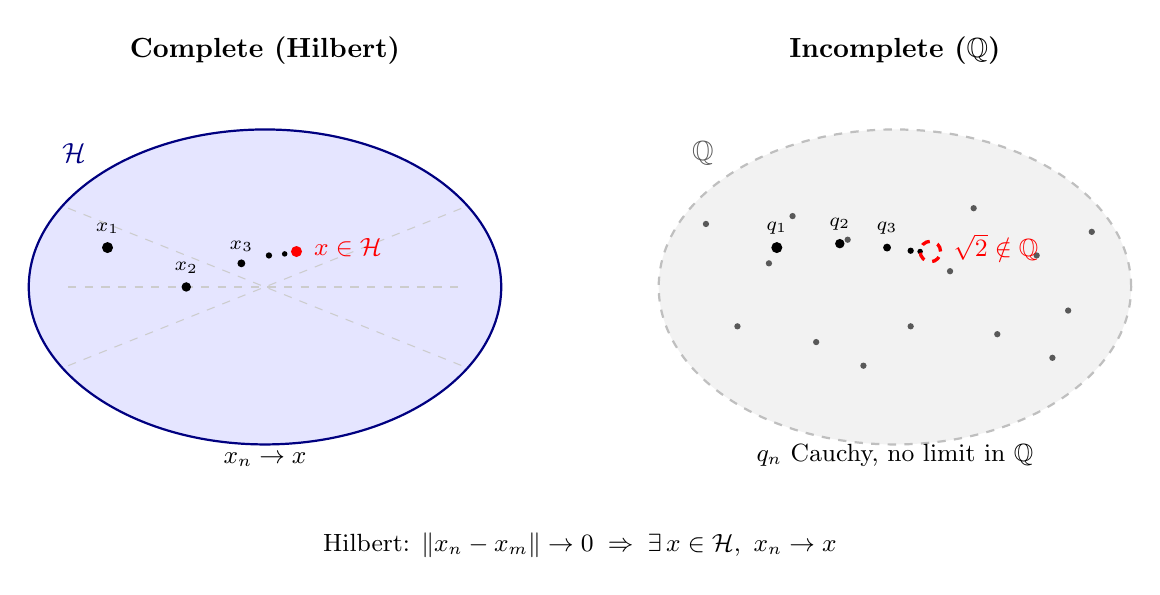
\begin{tikzpicture}[>=Latex]

  % LEFT — complete Hilbert space
  \begin{scope}[xshift=0cm]
    \node[font=\bfseries] at (0, 3.0) {Complete (Hilbert)};

    \filldraw[blue!50!black, fill=blue!10, thick] (0, 0) ellipse (3.0 and 2.0);

    % some "dimension lines"
    \draw[gray!40, dashed] (-2.5, -1.0) -- (2.5, 1.0);
    \draw[gray!40, dashed] (-2.5, 0.0) -- (2.5, 0.0);
    \draw[gray!40, dashed] (-2.5, 1.0) -- (2.5, -1.0);

    % sequence x_1, x_2, x_3 ... converging to x
    \fill[black] (-2.0, 0.5) circle (0.07); \node[font=\scriptsize, anchor=south] at (-2.0, 0.55) {$x_1$};
    \fill[black] (-1.0, 0.0) circle (0.06); \node[font=\scriptsize, anchor=south] at (-1.0, 0.05) {$x_2$};
    \fill[black] (-0.3, 0.3) circle (0.05); \node[font=\scriptsize, anchor=south] at (-0.3, 0.32) {$x_3$};
    \fill[black] (0.05, 0.4) circle (0.04);
    \fill[black] (0.25, 0.42) circle (0.035);
    \fill[red] (0.4, 0.45) circle (0.07);
    \node[font=\small, red, anchor=west] at (0.5, 0.5) {$x\in\mathcal H$};

    \node[font=\small, anchor=south] at (0, -2.4) {$x_n\to x$};
    \node[font=\bfseries, blue!50!black, anchor=west] at (-2.7, 1.7) {$\mathcal H$};
  \end{scope}

  % RIGHT — incomplete (rationals)
  \begin{scope}[xshift=8cm]
    \node[font=\bfseries] at (0, 3.0) {Incomplete ($\mathbb Q$)};

    \filldraw[gray!50, fill=gray!10, thick, dashed] (0, 0) ellipse (3.0 and 2.0);

    % rational points scattered (sparse)
    \foreach \x/\y in {-2.4/0.8, -2.0/-0.5, -1.6/0.3, -1.0/-0.7, -0.6/0.6, 0.2/-0.5, 0.7/0.2, 1.3/-0.6, 1.8/0.4, 2.2/-0.3, 2.5/0.7, -1.3/0.9, -0.4/-1.0, 1.0/1.0, 2.0/-0.9}{
      \fill[gray!70!black] (\x, \y) circle (0.04);
    }

    % approaching sequence
    \fill[black] (-1.5, 0.5) circle (0.07); \node[font=\scriptsize, anchor=south] at (-1.5, 0.55) {$q_1$};
    \fill[black] (-0.7, 0.55) circle (0.06); \node[font=\scriptsize, anchor=south] at (-0.7, 0.6) {$q_2$};
    \fill[black] (-0.1, 0.50) circle (0.05); \node[font=\scriptsize, anchor=south] at (-0.1, 0.55) {$q_3$};
    \fill[black] (0.20, 0.46) circle (0.04);
    \fill[black] (0.32, 0.45) circle (0.035);

    % Hole at limit
    \draw[red, very thick, dashed] (0.45, 0.45) circle (0.13);
    \node[font=\small, red, anchor=west] at (0.62, 0.5) {$\sqrt 2 \notin \mathbb Q$};

    \node[font=\small, anchor=south] at (0, -2.4) {$q_n$ Cauchy, no limit in $\mathbb Q$};
    \node[font=\bfseries, gray!70!black, anchor=west] at (-2.7, 1.7) {$\mathbb Q$};
  \end{scope}

  % bottom unifying caption
  \node[font=\small, anchor=north] at (4, -3.0)
    {Hilbert: $\|x_n-x_m\|\to 0\;\Rightarrow\; \exists\,x\in\mathcal H,\ x_n\to x$};
\end{tikzpicture}
\end{document}
